%%%%%%%%%%%%%%%%%%%%%%%%%%%%%%%%%%%%%%%%%%%%%%%%%%%%%%%%%%%%%%%%%%%%%%%%%%%%%%%
%%%%%%%%%%%%%%%%%%%%%%%%%%%%%%%%%%%%%%%%%%%%%%%%%%%%%%%%%%%%%%%%%%%%%%%%%%%%%%%
\section{Static Perspectives of Honey Bee Networks}
%%%%%%%%%%%%%%%%%%%%%%%%%%%%%%%%%%%%%%%%%%%%%%%%%%%%%%%%%%%%%%%%%%%%%%%%%%%%%%%
%%%%%%%%%%%%%%%%%%%%%%%%%%%%%%%%%%%%%%%%%%%%%%%%%%%%%%%%%%%%%%%%%%%%%%%%%%%%%%%

TODO write some intro

I analyzed a temporal network, consisting of three time-aggregated snapshots; these are referred to below as snapshot~1~($N=922$), snapshot~2~($N=978$) and snapshot~3~($N=922$). 
The snapshots are aggregated for ten hours (108,000 frames) starting at 8~a.m. and lasting until 6~p.m, see table~\ref{tab:networks} for details about the added bees per day,  figure~\ref{fig:ages} for the age distributions. Figure~\ref{fig:network-matching} shows the proportion of intersecting bees between each snapshot. This figure illustrates the stability of the network concerning its size. 

\begin{table}
\centering
\caption[Sampling period]{\textbf{Sampling period} Overview of the chosen day networks including the number of added bees and the time they were added to the hive.}
\vspace*{5mm}
\begin{tabularx}{\textwidth}{ccccccc}
\toprule
{} & 20.08.16 & 21.08.16 & 22.08.16 & 23.08.16 & 24.08.16 \\
\midrule
Network ID & 1 & - & 2 & - & 3 & \\
Number of added bees & 0 & 0 & 110 & 60 & 0 \\
Time added & - & - & 2~p.m. & 6~p.m. & - \\
\bottomrule
\end{tabularx}
\label{tab:networks}
\end{table}

\begin{figure}[htb]
	\centering
	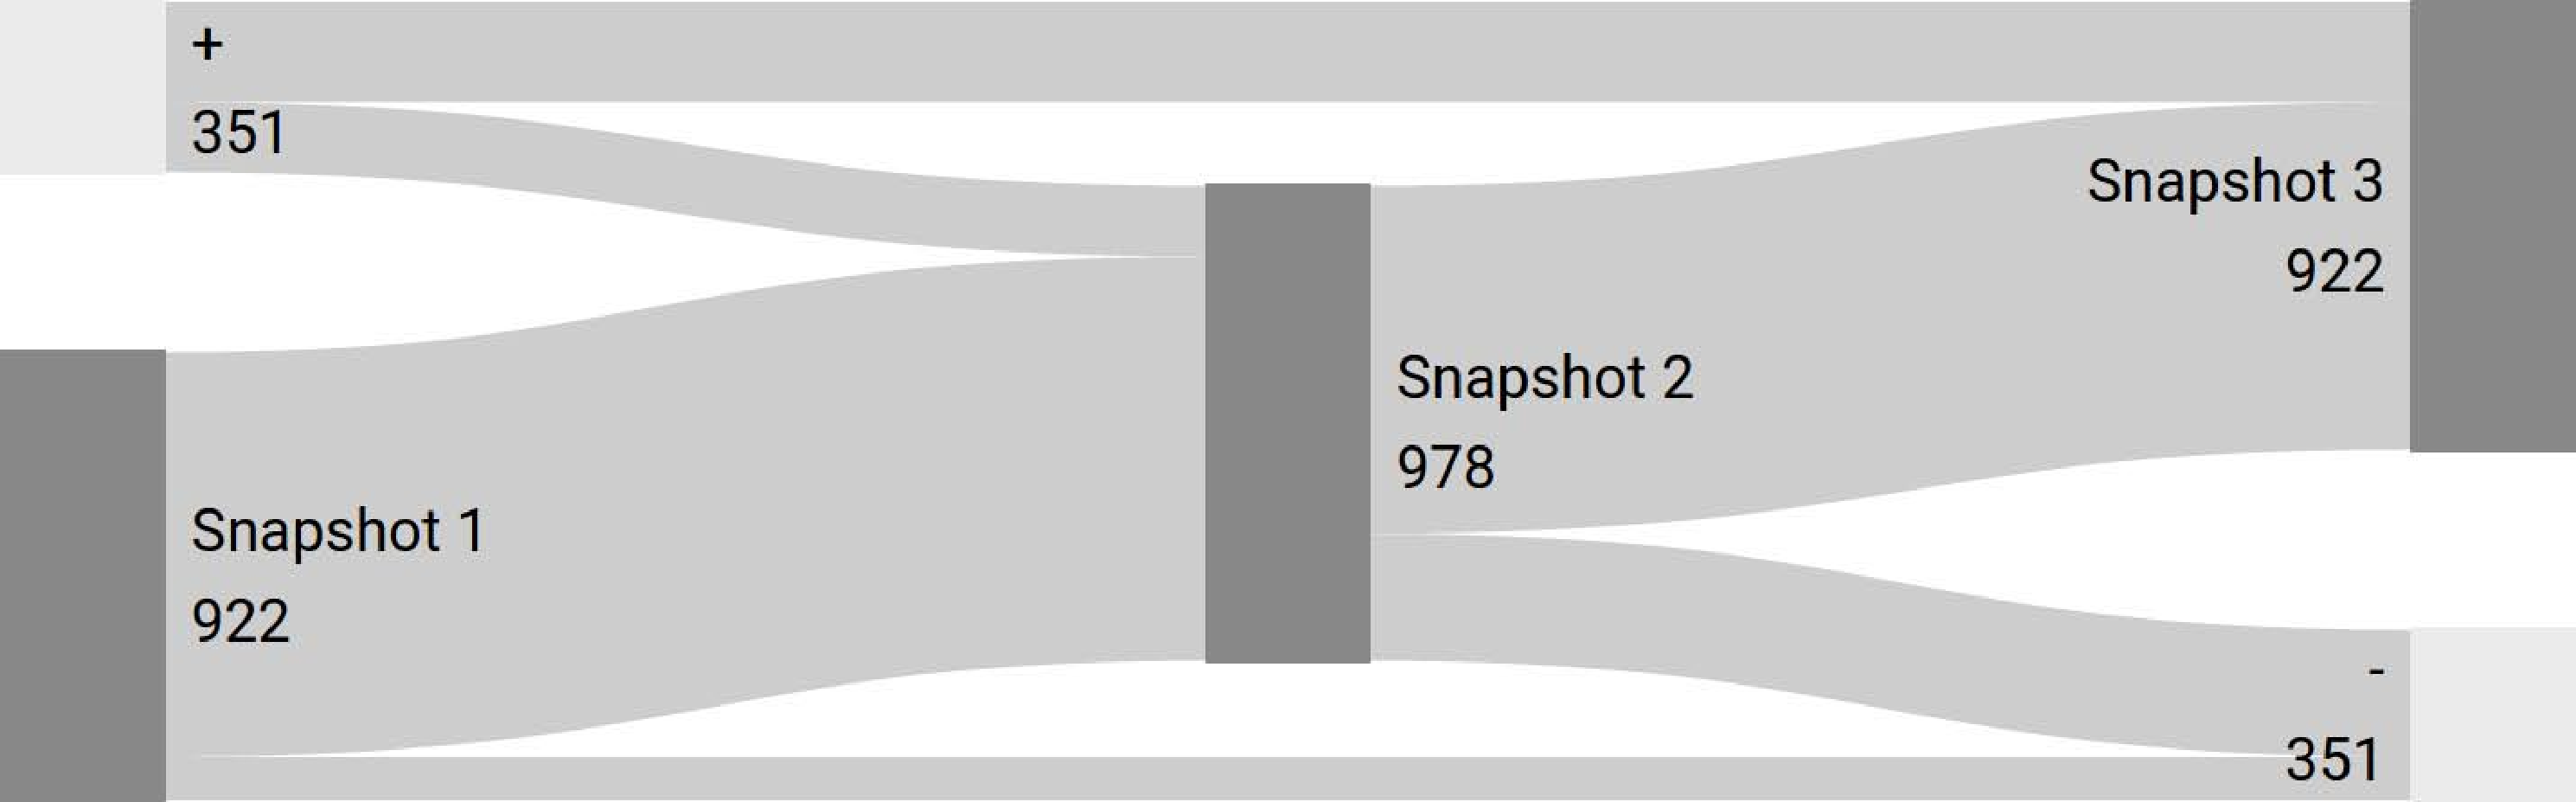
\includegraphics[width=.8\textwidth]{Figures/network_matching}
	\caption[Number of bees per snapshot]{\textbf{Number of bees per snapshot} This figure show the amount of bees for each snapshot and the proportion of intersecting bees between snapshots.}
	\label{fig:network-matching}
\end{figure}

%%%%%%%%%%%%%%%%%%%%%%%%%%%%%%%%%%%%%%%%%%%%%%%%%%%%%%%%%%%%%%%%%%%%%%%%%%%%%%%
\subsection{Properties of the Colony}
%%%%%%%%%%%%%%%%%%%%%%%%%%%%%%%%%%%%%%%%%%%%%%%%%%%%%%%%%%%%%%%%%%%%%%%%%%%%%%%
Each snapshot consists of one large component.
Table~\ref{tab:stats} summarizes basic network properties.
For all, the density $D$ is over 50\%.
The diameter $\langle d_{\texttt{max}} \rangle$ is three and the average shortest path length $\langle d \rangle$ is below two.
The global clustering coefficient $C_\Delta$ of all snapshots is higher than compared to an Erdös-Renyi random graph, averaged over 100 runs using the same number of nodes and edges.
The high clustering coefficient and the small diameter suggest a small-world network type.
On average, each bee is connected to at least 50\% of all other bees in the network.

Figure~\ref{fig:fVSd} shows a positive correlation between the frequency of interactions and the total duration of interactions (averaged).
 The weight of edges is the frequency of interactions.
The edge weight distribution is shown in figure~\ref{fig:edgeWdist}.
Most edges have a low weight; only a few edges have a high weight.
It seems that bees do not prefer individuals bees for interaction.

\begin{table}[htbp]
\small
\centering
\caption[Global network properties]{\textbf{Global network properties} $N$ number of nodes, $L$ number of links, $D$ diameter, $\langle d_{\texttt{max}} \rangle$ average path length, $\langle d \rangle$ diameter, $C_\Delta$ global clustering coefficient, $\langle k \rangle$ average degree and $\langle s \rangle$ represents the average strength, as introduced in section~\ref{sec:definitions}.}
\label{tab:stats}
\vspace*{5mm}
\begin{tabular}{rccccccccc}
\toprule
{} &  $N$ &   $L$ &  $D$ &  $\langle d_{\texttt{max}} \rangle$ &  $\langle d \rangle$ &   $C_\Delta$ & $\langle k \rangle$ &  $\langle s \rangle$ \\
\midrule
Snapshot 1 & 922 & 291179 & 0.69 & 3 & 1.32 &  0.79 & 631.62 & 5680.17 \\
Random 1  & 922 & 291179 & 0.69 & 2 & 1.31 &  0.69 & 631.62 & - \\ \midrule
Snapshot 2 & 978 & 256066 & 0.54 & 3 & 1.46 &  0.72 & 523.65 & 3977.94 \\
Random 2  & 978 & 256066 & 0.54 & 2 & 1.46 &  0.54 & 523.65 & - \\ \midrule
Snapshot 3 & 922 & 259421 & 0.61 & 3 & 1.39 &  0.75 & 562.74 & 4205.99 \\
Random 3  & 922 & 259421 & 0.61 & 2 & 1.39 &  0.61 & 562.74 & - \\
\bottomrule
\end{tabular}
\end{table}

\begin{figure}[htb]
	\centering
	\begin{subfigure}[b]{0.49\textwidth}
	\centering
	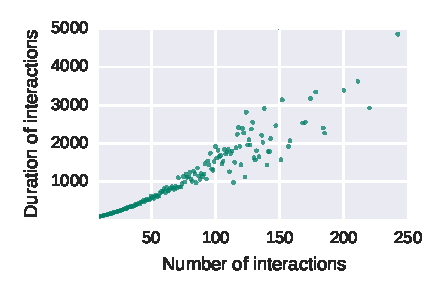
\includegraphics[width=1.0\textwidth]{Figures/n3-freqVSduration}
	\caption[Type of edge weights]{Type of edge weights}
	\label{fig:fVSd}
	\end{subfigure} 
	\begin{subfigure}[b]{0.49\textwidth}
	\centering
	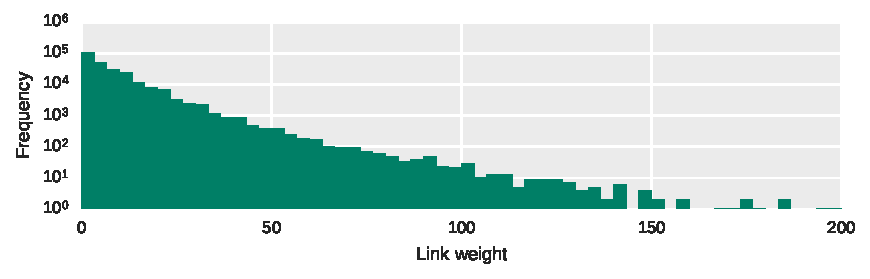
\includegraphics[width=1.0\textwidth]{Figures/n3-edgeWeightDist.pdf}
	\caption[Edge weight distribution]{Edge weight distribution}
	\label{fig:edgeWdist}
	\end{subfigure}
	\caption[Edge wights]{\textbf{Edge wights} }
	\label{fig:edges}
\end{figure}


Figure~\ref{fig:n3ageDist} shows the age distribution of the investigated snapshot. This distribution does not seem to follow any known distribution. It corresponds to the artificial tagging of bees. Consequently, bees of certain age groups are simply not present. The detection frequency of an individual bee is negatively correlated with its age (figure~\ref{fig:n3detfVSage}).


\begin{figure}[htb]
	\centering
	\begin{subfigure}[b]{0.33\textwidth}
	\centering
	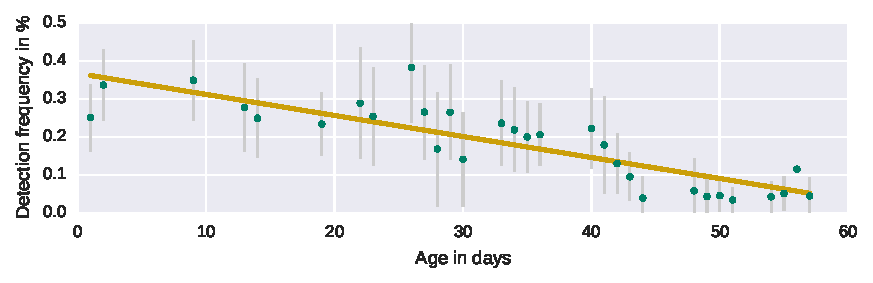
\includegraphics[width=1.0\textwidth]{Figures/n3_detFvsAge}
	\caption[]{}
	\label{fig:n3detfVSage}
	\end{subfigure} 
	\begin{subfigure}[b]{0.66\textwidth}
	\centering
	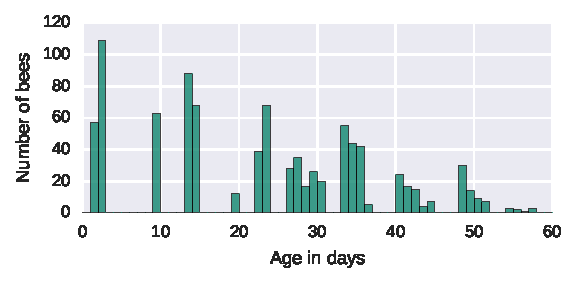
\includegraphics[width=1.0\textwidth]{Figures/n3_ages.pdf}
	\caption[]{}
	\label{fig:n3ageDist}
	\end{subfigure}
	\caption[X]{\textbf{X}}
	\label{fig:ageDetF}
\end{figure}


%%%%%%%%%%%%%%%%%%%%%%%%%%%%%%%%%%%%%%%%%%%%%%%%%%%%%%%%%%%%%%%%%%%%%%%%%%%%%%%
\subsection{Characteristics of Individual Bees}
%%%%%%%%%%%%%%%%%%%%%%%%%%%%%%%%%%%%%%%%%%%%%%%%%%%%%%%%%%%%%%%%%%%%%%%%%%%%%%%

Degree, Strength and Local Clustering Coefficient and \\
Betweenness and Closeness Centrality\\
\\
bimodal degree distribution\\
type of network: no scale free\\
todo plot in relation to age of bees\\
todo plot in relation to detection frequency\\

\begin{figure}[!htb]
	\centering
	\begin{subfigure}[b]{1.0\textwidth}
	\centering
	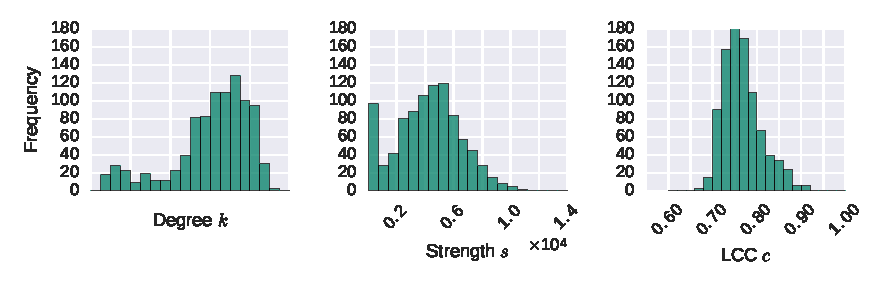
\includegraphics[width=1.0\textwidth]{Figures/n3-stat-degreeStrLCC}
	\caption[Distributions]{\textbf{Distributions}}
	\label{fig:n3-d-s-cc}
	\end{subfigure}
	\caption[Degree, strength and local clustering coefficient]{\textbf{Degree, strength and local clustering coefficient} xxx}
	\label{fig:n3-degreeStrLCC}
\end{figure}

[TODO]\\
in relation to age and detection frequency\\
closeness\\
betweenness\\

%%%%%%%%%%%%%%%%%%%%%%%%%%%%%%%%%%%%%%%%%%%%%%%%%%%%%%%%%%%%%%%%%%%%%%%%%%%%%%%
\subsection{Functional Groups within the Colony}
%%%%%%%%%%%%%%%%%%%%%%%%%%%%%%%%%%%%%%%%%%%%%%%%%%%%%%%%%%%%%%%%%%%%%%%%%%%%%%%
The leading eigenvector community detection algorithms revealed two communities, about the same size, the walktrap algorithm instead three communities (see table~\ref{tab:n3-communities}).
The communities correspond to separate age groups and are located in different regions on the comb (see figure~\ref{fig:n3-communities}). The younger communities are situated in the center and the old communities closer to the hive exit. The middle-aged community (only for walktrap) is located between and on the periphery. Table~\ref{tab:n3-pvalues2} shows the $p$-values for the two sampel KS-test.

\begin{table}[htb]
\small
\centering
\caption[Communities per algorithm]{\textbf{Communities per algorithm} Communities marked with * contain the queen. Age and standard deviation (SD) are measured in days. The queen and nine bees with a negative age are excluded from this analysis.}
\label{tab:n3-communities}
\vspace*{5mm}
\begin{tabular}{lcrrrrr}
	\toprule
	{}  & Community ID & Members & Proportion & Age & SD\\
	\midrule  
	\quad LE  & CY & $*381$  & 41.78\% & $13.15$ & $\pm13.50$ \\
	          & CO & $531$   & 58.22\% & $28.70$ & $\pm11.67$ \\
    \midrule 
	\quad WT & CY & $*229$  & 25.11\% & $6.55$  & $\pm10.36$\\
			 & CM & $298$  & 32.68\% & $25.08$ & $\pm11.97$\\
			 & CO & $385$  & 42.21\% & $29.29$ & $\pm11.44$\\
	\bottomrule
\end{tabular}
\end{table}
\begin{table}[htb]
\small
\centering
\caption[Kolmogorov-Smirnov test]{\textbf{Kolmogorov-Smirnov test} $p$-values for leading eigenvector (LE) and walktrap (WT)}
\label{tab:n3-pvalues2}
\vspace*{5mm}
\begin{tabular}{crrrrr}
	\toprule
	 Communities & LE p-value & WT p-value\\
	\midrule 
    CY, CO & 5.10e-66 & 5.51e-67\\
    CY, CM &          & 1.10e-95\\
    CM, CO &          & 1.98e-05\\ 
	\bottomrule
\end{tabular}
\end{table}

\begin{figure}[!htb]
	\centering
	\begin{subfigure}[b]{1.0\textwidth}
	\centering
	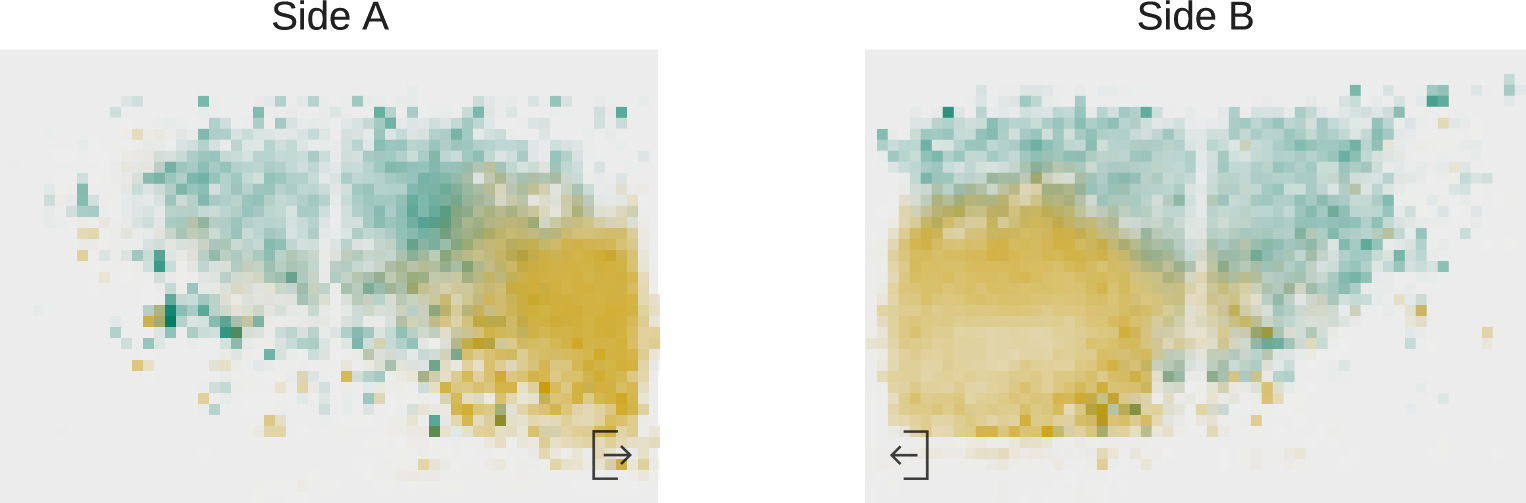
\includegraphics[width=1.0\textwidth]{Figures/le_network3}
	%\vspace{1pt}
	\end{subfigure} 
	\begin{subfigure}[b]{1.0\textwidth}
	\centering
	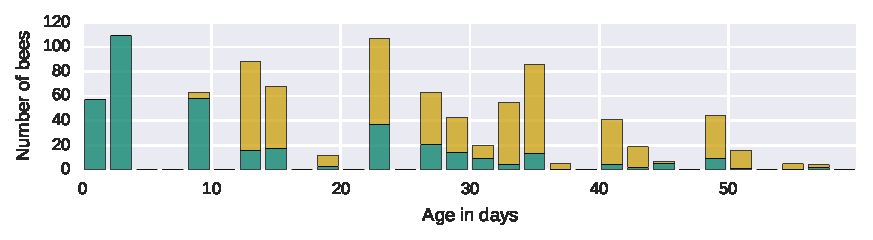
\includegraphics[width=1.0\textwidth]{Figures/n3-ageDistribution-LE}
	\caption[Leading eigenvector communities]{Leading eigenvector communities}
	\label{fig:n3ageLE}
	\end{subfigure}
	\begin{subfigure}[b]{1.0\textwidth}
	\vspace{5mm}
	\centering
	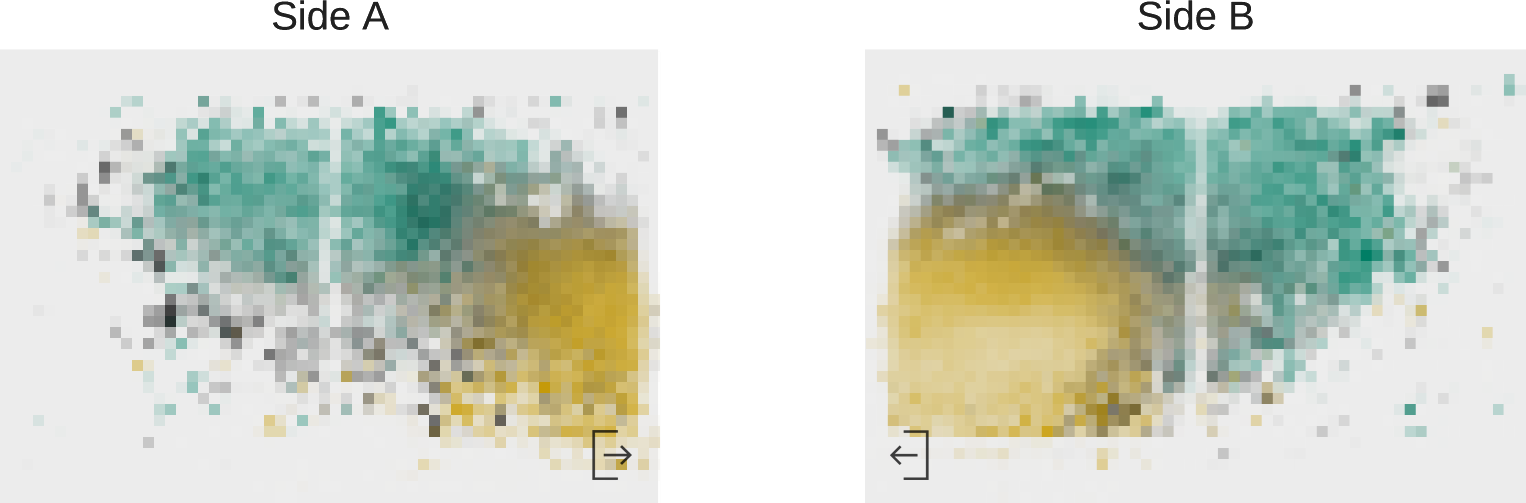
\includegraphics[width=1.0\textwidth]{Figures/wt_network3}
	\end{subfigure}
	\begin{subfigure}[b]{1.0\textwidth}
	\centering
	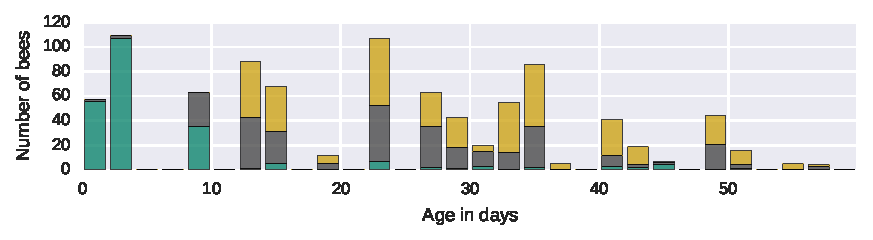
\includegraphics[width=1.0\textwidth]{Figures/n3-ageDistribution-WT}
	\caption[Walktrap communities]{Walktrap communities}
	\label{fig:n3ageWT}
	\end{subfigure}
	\caption[Age and spatial distribution of communities]{\textbf{Age and spatial distribution of communities} \emph{Green} represents the young community occupying the center are of the comb and \emph{orange} the old community, which is situated closer to the hive access. For walktrap the middle-aged community is depicted in \emph{gray} and is located inbetween.}
	\label{fig:n3-communities}
\end{figure}